\documentclass[letterpaper,11pt]{article}

\usepackage{amsmath} 
\usepackage{amsthm} 
\usepackage{amsfonts} %required for \mathbb
\usepackage{listings}
\usepackage{color}
\usepackage{listings}
\usepackage{graphicx}
\usepackage{setspace}
\usepackage{float}
\usepackage{hyperref}
\usepackage{courier}

\definecolor{lightgray}{gray}{0.95}
\hypersetup{
hidelinks}

\lstset{breaklines=true,
    language=Lisp,
    basicstyle=\footnotesize\ttfamily, 
    backgroundcolor=\color{lightgray},
}



\begin{document}
\title{MLang: Musical Language}
\author{Aditya Mukerjee, Nikhil Sarda, Nistha Agarwal, Sushmita Swaminathan}
\maketitle

\section{Introduction}

Aesthetics are by nature subjective and non-deterministic; as such, a programming language cannot fix this problem. But aesthetics are often determined by adherence to well-defined artistic conventions. Just as a simple Venician sonnet must have a fixed meter and rhyming scheme, musical compositions such as fugues, canons, and concertos must obey a well-defined structure specific to that musical form. When composing classical music, a deep understanding of music theory and strong grasp of music notation and grammar are required simply to create a piece compliant with the accepted contemporary musical structure - and that is all before beginning any part of the creative, artistic process. 

However, while the underlying theory is vast, these conventions are extremely well-defined. As a result, most of this process can be facilitated by use of a piece of software specific enough to be tailored to the individual piece of music at hand, yet powerful enough to allow the composer to break free of conventions when necessary, or even to redefine or extend the set of rules. Traditionally, this software is implemented as a graphical frontend to standard music notation. The creators of MLang believe that undermines the power of music. Music is itself a language, and a composition is simply an application of the language, just as a program is an application of a programming language.

The language we have described is simply the language of music - simple and minimal, yet powerful. The same is true of homoiconic functional programming languages, which made the selection of a programming paradigm MLang rather clear. Homoiconic functional languages are simple, yet highly powerful, and they derive this power through their modularity.

MLang is a language that helps its users compose music by writing and compiling programs. It is a homoiconic functional language that is simple,
yet highly powerful, and modular. Many of MLang's features are similar to a functional programming language like LISP. 
Thus, familiarity with functional programming languages and a basic knowledge of music is preferred but not required.


\subsection{Modularity}
Music itself is highly modular. Not only is it common for sections of music to be repeated exactly within a given piece of music, but it is often expected that variations on these sections be repeated within the same composition. Subsequently, these sections may included in later compositions by other authors. All music is thus, in some sense, derivative - it is the nature of the art form.  

MLang exposes this modularity, intrinsic in music, and turns it from a barrier to entry into a tool for the beginning composer (and instructors of music composition). Like standard music composition software, MLang allows composers to create music from scratch, by defining notes individually.  Thus, a user familiar with traditional music notation would have little trouble adjusting to MLang. Most music composition software provides this feature and little else. MLang, however, takes this a step further, by allowing the composer to extract arbitrary elements from that music and bundle these elements together into a module.

\subsection{Metaprogramming}
MLang allows the user to incorporate other pieces of MLang code - which are playable music files - into their own code as modules. A module is not limited to being just a complete musical phrase, such as a measure, a note, or an entire movement. It may be an attribute of the music, such as the key, time signature, or timbre - these attributes are not necessarily observed (ie, heard) in just a single section of the composition, but rather, they are woven into the composition as a whole. 


\subsection{Homoiconicity}
A language is said to be homoiconic if a representation of programs written in it are also a data structure in a primitive type of the language itself. In MLang, the only primitive is a list of musical notes, or a function. However, because functions are themselves defined by a list, everything in MLang, including the code itself, is a representation of a series (list) of notes. Modules, the higher-level data structures, are themselves recursively composed of other modules or of primitives (notes). So the code itself has a recursive representation as a primitive datatype. For MLang, the elementary datatype is an m-expression. We define an M-expression recursively as 
1. a musical note, or
2. an expression of the form (x . y) where x and y are m-expressions.
Note the analogous relationship between an m-expression and an s-expression.

\subsection{Functional}
MLang treats computation (generation of music) as simple evaluation of m-expressions and avoids state and mutable data for many transactions. MLang is heavily influenced by the syntax and semantics of Lisp and its variants, though the interpreter itself is written in OCaml. MLang is strongly typed and dynamic.


\section{Language Tutorial}

\subsection{Conventions}

In this tutorial > refers to the command line prompt and {> refers to the
output of the MLang command.

\subsection{Data Types}
The basic data type in MLang is an MNote. An MNote is a list of length 1
and can be thought of as a function with no arguments.
An MNote can be represented as 

\lstset{breaklines=true,language=Lisp}
\begin{lstlisting}
(%rest %A %octave), 
\end{lstlisting}

where A refers to any musical note.
\lstset{breaklines=true,language=Lisp}
\begin{lstlisting}
> (label A (8 A 3))
\end{lstlisting}

In order to play the above, we can write

\lstset{breaklines=true,language=Lisp}
\begin{lstlisting}
> (label A (8 A 3))
> (read-file stdlib.mlang)
> (midge-export test.mg ((100 4 4) ((piano_grand_ac 80 1 (A)))))
> (label A (8 A 3))
\end{lstlisting}
The midge-export function takes two arguments, the filename and the song m-expression. A song is represented as a head and a body. The head contains
information such as tempo and time signature. The body consists of several channels. A channel has information such as the instrument, volume, repetitions and the notes themselves.

In the above example, the head is (100 4 4) which represents a tempo of 100 bpm and a time signature of 4/4.
There is a single channel and a single note. The instrument of choice is grand piano, volume is 80 and the A note on the 3rd octave is played once
with a 1/8 rest.

Go back to the terminal and you will see a test.mg file has been created. In order to play it type

\lstset{breaklines=true,language=bash}
\begin{lstlisting}
# midge test.mg
# banshee test.mid

\end{lstlisting}

\subsection{Input and Output}
The input for MLang would consists of codes written at the command line or as part of a fille with the .mlang extension.
The code is a series of mexpressions that represent notes, functions and other metadata.
On compilations, the program would produce a file with the .mg extension which can be postprocessed with Midge in order to produce a .mid file.

\subsection{MLang Expressions}

The common form of an MLang expression is a function application given by the syntax

\lstset{breaklines=true,language=Lisp}
\begin{lstlisting}
(function arg1 arg2 ...)
\end{lstlisting}
where the arguments can be MNotes or other functions.

MLang expressions are case insensitive: (A 100) and (a 100) mean the same

\subsection{Functions as values}

Since MLang is a homoiconic language, functions can be treated as data that can be passed around.
In MLang, all functions are evaluated to notes. Thus every function eventually is evaluated to a string of notes that forms the midi.

\lstset{breaklines=true,language=Lisp}
\begin{lstlisting}
> (MAPCAR TRANSPOSE ((4 A 3) (4 B 3) (4 C 3)))
\end{lstlisting}

where the arguments can be MNotes or other functions.
For instance, TRANSPOSE is a function that is passed as an argument to another function, in this case MAPCAR. MAPCAR applies TRANSPOSE to each
of the MNotes in the third m-expression

Another example
\lstset{breaklines=true,language=Lisp}
\begin{lstlisting}
> (read-file stdlib.mlang)
> (LABEL BASSPHRASE
  	 (CONCAT (REPEAT4 (3 B 16)) (REPEAT4 (3 A 16)) (REPEAT4 (3 G 16)) (REPEAT4 (3 A 16))))
\end{lstlisting}

Here REPEAT4 is a lambda function defined in stdlib.mlang. It takes a parameter and returns an mexpression containing it 4 times. CONCAT takes
all of these m-expressions and concatenates them.


\subsection{Writing Your First MLang Program}
Here is an example .mlang program that plays the first few notes of Happy Birthday

\lstset{breaklines=true,language=Lisp}
\begin{lstlisting}
((read-file stdlib.mlang)
	(label head
	       (42 4 4))
	(label phrase1
	       ((3 g 4) (3 g 4) (3 a 4) (3 g 8)))
	(label channel1
	       (bass_ac 96 1 phrase1))
	(MIDGE-EXPORT
		happy.mg (head (channel1))))
\end{lstlisting}

The first statement is used to load the standard library.

The label keyword is used to bind a string with an m-expression. Here we have bound head with the mexpression (42 4 4).
We have then defined the first phrase which consists of 4 notes. The label channel1 is made up of phrase1. An m-expression is then created
which is fed into midge-export.

In order to play this song from the commandline type
\lstset{breaklines=true,language=bash}
\begin{lstlisting}
# ./mlang < happy.mlang && midge happy.mg && banshee happy.mid
\end{lstlisting}

MLang is portable in the sense that it does not depend upon the machine’s hardware for its execution.

\subsection{Working with higher-order functions}


Here we show how one can use higher-order functions in order to write compact mlang programs.

\lstset{breaklines=true,language=Lisp}
\begin{lstlisting}
> (LABEL REVERSECHANNEL
       (LAMBDA (X)
                      ((CAR X) (NTH 1 X) (NTH 2 X) (REVERSE (NTH 3 X)))))

\end{lstlisting}
This is a function that reverses the fourth mexpression in a given mexpression. For instance

\lstset{breaklines=true,language=Lisp}
\begin{lstlisting}
> (REVERSECHANNEL (1 2 3 (A B C)))
(1 2 3 (C B A))
> (REVERSECHANNEL (1 2 3 (A B C)))
\end{lstlisting}
Let us make use of REDUCE, our version of a left fold.

\lstset{breaklines=true,language=Lisp}
\begin{lstlisting}
> (REVERSECHANNEL (1 2 3 (A B C)))
> (LABEL GG (LAMBDA (X Y) (CONCAT X Y)))
> (REDUCE GG ((A B) (C D)) nil)
(nil A B C D)

\end{lstlisting}
REDUCE takes three parameters, a function that takes two arguments (accumulator and element) followed by an mexpression and the initial value.
It then proceeds to left fold the mexpression using the given function.

		      
\section{Language Reference Manual}


\subsection{Lexical Conventions}

 Aditya: Please fill up


\subsection{Character Set}


Mlang programs are written in ASCII character set.


\subsection{Identifiers}

In MLang, an identifier is a string that starts with a letter or an underscore, and consists
of a sequece of letters, digits, and underscores. Identifiers are case insensitive.


\subsection{Keywords}


The following keywords are reserved 


\begin{list}{}{}
\item \texttt{  QUOTE }
\item \texttt{ CAR }
\item \texttt{ CDR }
\item \texttt{  SETCAR }
\item \texttt{ SETCDR }
\item \texttt{ CONS }
\item \texttt{  EQUAL }
\item \texttt{ ATOM }
\item \texttt{ COND }
\item \texttt{  IFELSE }
\item \texttt{  LAMBDA }
\item \texttt{  LABEL }
\item \texttt{ READ-FILE }
\item \texttt{ WRITE-FILE }
\item \texttt{  LENGTH }
\item \texttt{  NTH }
\item \texttt{  LAST }
\item \texttt{  MAPCAR }
\item \texttt{  REDUCE }
\item \texttt{  INC }
\item \texttt{ DEC }
\item \texttt{  COMBINE }
\item \texttt{ REVERSE }
\item \texttt{ CONCAT }
\item \texttt{ MIDGE-EXPORT }
 \end{list}
These are simply functions whose behavior has been defined in OCaml.

\subsection{Types}


The basic type in MLang is the Mexp which is a cell. The Mexp is defined as

\lstset{breaklines=true,language=ml}
\begin{lstlisting}
type ('a, 'b) cell = { mutable car: 'a; mutable cdr: 'b }

type t = Atom of string
  | Cons of (t, t) cell
  | Func of (t -> (string, t) Hashtbl.t -> t)
  | Lambda of t * t
  | Null

\end{lstlisting}


Thus our language only provides symbol atoms (no integers, strings, etc)
and cons cells. It is dynamically scoped.


\subsection{M-expressions}


The following are valid m-expression
\lstset{breaklines=true,language=Lisp}
\begin{lstlisting}
> (1 2 3 4)

> (A B C)

> (LENGTH (1 2 3))

> (LABEL A (a l p h a))

\end{lstlisting}
\subsection{Grammar}


The grammar of Mlang is incredibly simple.
It has expressions, which are symbolic identifiers, and lists.
A list is a left parenthesis followed by some number of expressions (separated by spaces) followed by a right parenthesis.

expr:   ID | list
list:   ( seq )  
seq:       | expr seq

\subsection{Higher-order functions}

\begin{tabular}{|c||c|}
    \hline
    Function & Description\\
    \hline
CONS		 & Given note A and a list of notes L, prepend A to L \\
CDR 	  	 & Given a list L, return the second element of the first cons cell \\
CAR 	  	 & Returns the first element in the list\\
QUOTE  	 & Creates a list of elements formed of the arguments\\
    SETCAR	 & Set CAR, evil, added for completeness (do not use)\\
SETCDR	 & Set CDR, ditto\\
EQUAL  	 & Checks for symbolic equality of two mexpressions\\
ATOM	  	 & Represents a single note\\
COND		 & Evaluates a series of conditions\\
 IFELSE	 & Conditional\\
 LAMBDA	 & Anonymous function definition\\
 LABEL      	 & Used to define new functions \\
 READ-FILE  	 & Reads commands from an input file\\
 WRITE-FILE 	 & Writes the output to a file\\
 LENGTH     	 & Used to find the length of the list\\
 NTH	       	 & Finds the nth element in a list\\
 LAST       	 & Finds the last element in a list\\
 MAPCAR     	 & Applies the function to every element in the list	\\
 REDUCE     	 & Fold left\\
 INC	       	 & Increments integer atom\\
 DEC	       	 & Decrements integer atom\\
 COMBINE    	 & Zips up two mexpressions\\
 REVERSE    	 & Reverses a given list\\
 CONCAT     	 & Concatenates mexpressions\\
 MIDGE-EXPORT & See the next section\\
    \hline
\end{tabular}


\subsection{Midge backend}


MIDGE-EXPORT takes 2 arguments, the name of the output file and an m-expression representing the song of the midi file. 

\lstset{breaklines=true,language=Lisp}
\begin{lstlisting}
(MIDGE-EXPORT name.mg SONG)
\end{lstlisting}
The song is an m-expression represented as:

\lstset{breaklines=true,language=Lisp}
\begin{lstlisting}
(HEAD BODY)

HEAD -> (TEMPO SIGNATURE_NUMERATOR SIGNATURE_DENOMINATOR)
\end{lstlisting}

Head consists of the song of the tempo, numerator and denominator of the time signature.

\lstset{breaklines=true,language=Lisp}
\begin{lstlisting}
BODY -> (CHANNEL1 CHANNEL2 CHANNEL3....)

\end{lstlisting}
A body is a sequence of channels.

\lstset{breaklines=true,language=Lisp}
\begin{lstlisting}
CHANNEL1 -> (INSTRUMENT VOLUME REPETITION (NOTE1 NOTE2 NOTE3...))

\end{lstlisting}
A channel is represented by its instrument, volume in the mix, the number of times it must be repeated and finally, the sequence of notes.

\lstset{breaklines=true,language=Lisp}
\begin{lstlisting}
NOTE1 -> (rest note-literal octave)

\end{lstlisting}
For instance the A note on 3rd octave played as a quarter note can be
represented as

\lstset{breaklines=true,language=Lisp}
\begin{lstlisting}
(4 A 3)
\end{lstlisting}

\section{Project plan (Sushmita Swaminathan, Project manager)}

The goal of the project was to create a programming language for music, one that is Turing complete as well as homoiconic and functional.


\subsection{Testing Model}
We divided the project into a number of sub-tasks that would be performed repeatedly until the final product was obtained. These stages were
Goal Forming/Reassessing, Compiler Design, Design implementation/Development and Testing.

\subsection{Goal Forming/Reassessing}
As the first step of the project, the main goals and objectives were defined and communicated to all members of the team. Subsequently, at regular intervals these goals were reassessed to ensure that their relevance was still maintained. Also, new goals were formulated, while some ideas that were not pertinent were discarded. While the main goal was to develop a language that would play music, some of the smaller goals that were set for the team included getting familiar with Ocaml and Lambda Calculus.

 \subsection{Compiler Design}
This phase was very critical, since it defined the structure of the entire project. We decided on Ocaml as our compiler language. The reason was
that since we were developing a functional language, it made more sense to use a functional language to implement it too. Another reason was that
most DSLs implemented in the industry are built on top of functional languages such as Haskell and ML so an exercise in writing a significant
project in OCaml would prove beneficial in the long run as well.
Since one of our design goals was homoiconicity, we had to be very careful while designing the language semantics. Thus, we decided to base our
language on Scheme/Lisp as it is the most tried and tested homoiconic language. 
For the backend, we decided to use Midge for creating the .midi files that would eventually play the music. This was chosen in order to keep our
implementation sandbox pure as Midge was the least intrusive of all the options.

 \subsection{Development}
In this phase, the designs were translated into executable code. The first implementations were of the lexer and parser, followed by the creation of an MLang environment and associated built-ins. New ideas that emerged during this time were reassessed.

 \subsection{Testing}
Closely following the development, we also tested the created applications.  The process of development and testing followed cyclically till there were no further issues to be resolved. This ensured that any bugs in the program could be immediately detected and fixed.



\section{Roles and Responsibilities}

\subsection{Project Manager (Sushmita Swaminathan)}
Keep end objective always in sight
Project design and implementation issue tracking and management
Ensuring constant communication among team members
Maintain regular checks to assess progress and pace of the project
Managing team issues
Contributing to the design and development in a technical role

\subsection{Language Guru (Aditya Mukerjee)}
Principal contributor to the design of the language
Provide domain expertise that helps clarify doubts and issues that arise implementation
Offer suggestions to improve on existing design and implementation
Suggest new features or offer alternatives to be incorporated in the existing language design
Technical contributor the design and development of the language

\subsection{System Architect/Integrator (Nikhil Sarda)}
Suggest and decide on the compiler language for MLang
Principal architect of the MLang environment
Identify the critical modules to be implemented and issues with language design that need rethinking
Ensure code flow through all the modules without break
Main deciding factor in accepting or rejecting design decisions based on development limitations

\subsection{System Tester (Nishtha Agarwal)}
Worked in tandem with the Architect to ensure code flow without breaks
Identify pain-points in the code that could lead to potential errors
Develop test cases for all the implemented modules
Exhaustive testing of all modules to ensure their functioning
Communicate all errors to the team and receive clarifications on implementations and bugs
Develop a test suite that tests for errors when the Make is run

\section{Implementation stylesheet}

These are some of the implementation rules that the team followed while developing the project

\subsection{Parentheses}
Balanced parenthesis are the most important syntactic feature of MLang. All parenthesis in MLang should be of the form “(“ or “)”, with every opening parenthesis having a matching closing parenthesis.  

All remaining closing parentheses should occur on the same line as the last command. For ex:

\begin{lstlisting}
(LABEL FF
(QUOTE A))  
is correct
(LABEL FF 
	(QUOTE A)
)
\end{lstlisting}
should be avoided

\subsection{Line separation}
Every block of function implementation should be separated from the next by a line separation. This facilitates readability of the code.
Indentation

Proper indentation must be maintained. When starting a new line, move the indentation to the position of the last non-matched parenthesis in the previousline.
 
\subsection{Keywords}
All the MLang functions should be written in uppercase. MLang is case-sensitive and will not recognize lowercase functions. Auto-indentation and auto-capitalization features are offered by the MLang-mode in emacs, which can be used.

\subsection{Comments}
“;” should be used for comments. Wherever required appropriate comments should be detailing the method implemented.

\subsection{File extensions}
All MLang files, including the standard package, should have a .mlang extension. 

\subsection{Function Names}
Function names should not be arbitrary, but should be indicative of the operations being performed.

\subsection{Timeline}

\subsubsection{January}

\begin{itemize}
\item Discussions and Brainstorming on language ideas
\item Finalized language to be implemented as MLang and the type of language to be functional
\item Preliminary Goal Setting – Evaluating implementation choices (OCaml, Java, C),
\item Understading Lambda Calculus and functional programming features
    \end{itemize}

\subsubsection{February}

\begin{itemize}
\item Finalize compiler language to be Ocaml	
\item Develop design implementation strategies for MLang
\item Finalize language features such as syntax – to maintain Lisp like syntax, M-expressions to parse MLang code
\item Language Whitepaper
\item Implementation of lexer and parser modules

    \end{itemize}
\subsubsection{March}

\begin{itemize}
\item Develop built-ins for MLang
\item Create MLang environment, execute basic function and simple tests for errors
\item Consider Midge as a possible back-end for creating the music
\item MLang Reference Manual
\item Language Tutorial
\item Working Midge back-end written

    \end{itemize}

\subsubsection{April}

\begin{itemize}
\item Java (JFugue) offered as alternative for music creations
\item Team decides to stick with Midge for creating the .midi files
\item Midge back-end completed
\item Hello World works! Demo given to Aho in class.
\item More built-in functions (SETCAR, SETCDR, IFELSE, CONCAT) added
\item Sample MLang programs written
\item Exhaustive testing of functions begins

    \end{itemize}

\subsubsection{May}

\begin{itemize}
\item Midge function, MIDGE-EXPORT added
\item Built-ins such as REVERSE, NTH, LENGTH,COMBINE, READ-FILE,WRITE-FILE added
\item MLang stdlib defined with functions such as TRANSPOSEUP, TRANSPOSEDOWN, NUMNOTES, REVERSEBODY
\item Songs paranoid.mlang, reaper.mlang, happy.mlang created
\item Mlang-mode defined for emacs
\item Testing and bug-fixing continue
\item Project Report
\item Project Presentation

    \end{itemize}


\subsection{git Log}
Note: This is the log for the testing branch; the full log is available on Github.
\lstinputlisting{gitlog.log}

\section{Translator Architecture (Nikhil Sarda, System Architect)}
\subsection{Architecture}

        \begin{figure}[H]
            \centering
            \makebox[0cm]{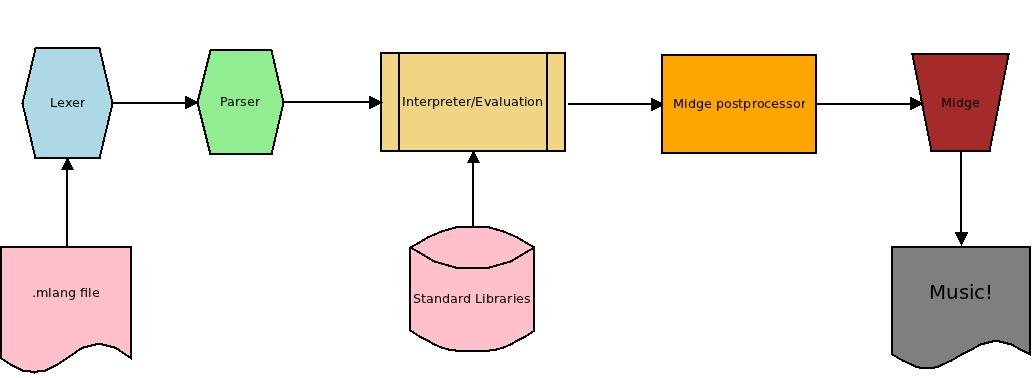
\includegraphics[scale=.2]{ArchitectureDiagram.jpg}} 
        \end{figure}
The above is a high-level overview of the architecture of the MLang compilation process. The mlang program goes through the lexer and parser that
generate an ML representation of a m-expression. This representation is then evaluated and processed into an m-expression that can be understood
by the Midge backend. If at this point definitions present in the standard library are needed, they are loaded as well.
We have defined some in built functions as well as several functions written in MLang itself. Functions written in OCaml were done so in order to
take advantage of tail-call optimization and other performance reasons. However, keeping in line with the design goal of MLang as a homoiconic
music language, NO music specific function was written in OCaml. M-expression evaluation is quite straightforward. As we walk the AST, we pattern-
match specific m-expression forms. For instance, if we encounter an atom, we check it against a hash-table that represents all the environment
variables and their respective mexpression bindings. If a binding exists, it is replaced in place of that atom and evaluated with the rest of the
m-expression treated as arguments. If not, we move on to the next m-expression. Forms such as lambdas and function calls are evaluated similarly.
The backend then generates intermediate .mg files which is then converted to MIDI. If a MIDI synthesizer is present on the system, it can be played 
with any conventional player.

\subsection{Interesting technical notes}

MLang has no side-effects. The only IO it can do is through the READ-FILE, WRITE-FILE and EXPORT-MIDGE keywords. This functionality piggy-backs on
OCaml.

Evaluation in MLang is eager.

Garbage collection in MLang piggy-backs on the OCaml run-time.

\subsection{Module Contributions}
Nikhil Sarda: Lexer, parser, most of the interpreter/evaluator, midge backend, standard library functions (translation of standard library from Lisp to pure Mlang.)
Sushmita Swaminathan: READ-FILE, WRITE-FILE function
Aditya Mukerjee: Standard library functions (pure Lisp lambda implementation), datatype fixed-point combinator, testing framework, fixes to the interpreter, repository sanitization


\section{Development and run-time environment (Nikhil Sarda)}

\subsection{Environment}


We used OCaml for all our development purposes. The compiler used was The Objective Caml toplevel, version 3.12.1 along with the Batteries Included
standard library. We used GNU Make for our build process after evaluating and rejecting OCamlBuild. Shell scripts were used as glue.
For most editing tasks, we used vim and emacs. Keeping in line with our preferences for extensible and fast editors instead of full
blown IDEs, we developed an emacs-mode for MLang as well. For version control, we used Git. This allowed us to work with multiple branches in a
completely distributed manner and allowed for easy merging when we needed to integrate the various components that different people were working on.
We used Github for source code hosting as well as for issue tracking. Email was used extensively for technical discussions.

\subsection{Build Process}
\lstset{language=bash}
\subsubsection{Makefile}
\begin{lstlisting}
OCAMLC=ocamlc
OCAMLOPT=ocamlopt
OCAMLDEP=ocamldep
INCLUDES=
OCAMLFLAGS=$(INCLUDES) -g
OCAMLOPTFLAGS=$(INCLUDES)

MAIN_OBJS=mexp.cmo midge.cmo parser.cmo lexer.cmo symtab.cmo environment.cmo builtins.cmo main.cmo

mlang: .depend $(MAIN_OBJS)
	$(OCAMLC) -o mlang $(OCAMLFLAGS) $(MAIN_OBJS)

.SUFFIXES: .ml .mli .cmo .cmi .cmx .mll .mly

.mll.ml:
	ocamllex $<
.mly.ml:
	ocamlyacc $<
.ml.cmo:
	$(OCAMLC) $(OCAMLFLAGS) -c $<

.mli.cmi:
	$(OCAMLC) $(OCAMLFLAGS) -c $<

.ml.cmx:
	$(OCAMLOPT) $(OCAMLOPTFLAGS) -c $<

testmlang: $(MLANG)
	./run_test.sh test_repl_input.txt

clean:
	rm -f mlang
	rm -f *~
	rm -f *.cm[iox]
	rm -f parser.ml parser.mli
	rm -f lexer.ml

parser.cmo : parser.cmi
parser.mli : parser.mly
parser.ml : parser.mly


.depend:
	$(OCAMLDEP) $(INCLUDES) *.mli *.ml *.mly *.mll > .depend

include .depend
\end{lstlisting}

\subsubsection{.depend}
\begin{lstlisting}
\end{lstlisting}

\subsubsection{.depend}
\lstset{language=bash}
\begin{lstlisting}
builtins.cmo: symtab.cmo mexp.cmo environment.cmo midge.cmo
builtins.cmx: symtab.cmx mexp.cmx environment.cmx midge.cmx
environment.cmo: mexp.cmo
environment.cmx: mexp.cmx
main.cmo: symtab.cmo mexp.cmo environment.cmo builtins.cmo midge.cmo
main.cmx: symtab.cmx mexp.cmx environment.cmx builtins.cmx midge.cmx
midge.cmo: mexp.cmo
midge.cmx: mexp.cmx
mexp.cmo:
mexp.cmx:
symtab.cmo: mexp.cmo
symtab.cmx: mexp.cmx
\end{lstlisting}

\subsubsection{run\_test.sh}
\lstset{language=bash}
\begin{lstlisting}

#A very basic, very hacky unit testing framework

filename=$1

repl_test()
{
    failed=0
    echo "Begin tests"
    while read p; do
        mlang_input=$(echo $p | cut -d '|' -f1)
        mlang_output=$(echo $mlang_input | ./mlang  | cut -b 1-2 --complement | head -n 1| sed 's/^ *//g' | sed 's/ *$//g')
        desired_ouput=$(echo $p | cut -d '|' -f2 | sed 's/^ *//g' | sed 's/ *$//g')
        if [ "$mlang_output" = "$desired_ouput" ]
        then
            echo ".............passed $p"
        else
            echo "!FAILED: $mlang_input produced $mlang_output instead of $desired_ouput"
            failed=`expr $failed + 1`
        fi
    done < $filename
    exit $failed
    
}

repl_test $filename

\end{lstlisting}


\subsection{Runtime Environment}
Instead of creating a separate compiler, we leveraged the REPL to act as a compiler. This was accomplished by adding a keyword MIDGE-EXPORT, which
creates the respective .mg file. We then post-process it using midge and run it with our music player of choice. For instance, if you wished to
compile a .mlang program, you would write

\lstset{language=bash}
\begin{lstlisting}
# ./mlang < my-program.mlang && midge my-program.mg && banshee my-program.mid
\end{lstlisting}
To simplify this, we created a small shell script called mlangc which does all of this automatically.

Please note that in order to run an mlang program, the user must install Midge as well as a MIDI synthesizer. Midge has a further dependency on
Perl.

\section{Test Plan(System Tester, Nishtha Agarwal)}


\subsection{Testing MLang Constructs: UNIT AND REGRESSION TESTS}

Since MLang depends heavily upon lambda expressions (S-exp that is), the basic test consisted of creating a list:


\lstset{language=Lisp}
\begin{lstlisting}
	(LABEL FOO (CONS A B))

\end{lstlisting}
Once a list is successfully created, tests on these lists were carried out. While most of the functions like CAR and CDR work in a similar fashion as that of LISP, many other were defined using LABEL.

\lstset{language=Lisp}
\begin{lstlisting}
	(LABEL TRUE (LAMBDA (X) (LAMBDA (Y) X)))

\end{lstlisting}
The built-in functions are defined in OCaml, the language of the compiler. OCaml being a functional language, the task of testing the functions thus defined was to check if the given expressions evaluate to a correct S-exp.

A Simple Example:
\lstset{language=Lisp}
\begin{lstlisting}

	(quote(a d d f))
 evaluates to (a d d f)

\end{lstlisting}

Moving on, the power of MLang lies in the nesting of functions i.e. an entire program can be written as just a single function!
To test this, a not-so-basic example involving the concept of functions-of-function:

\lstset{language=Lisp}
\begin{lstlisting}
	(quote (a b c (cdr (a b c))))
 evaluates to (a b c (b c))

\end{lstlisting}

Testing the conditional constructs:

\lstset{language=Lisp}
\begin{lstlisting}
	((LABEL TRANSPOSE
      (LAMBDA (X)
              (COND ((EQUAL (CAR (CDR X)) C) ((CAR X) C+ (LAST X)))
                    ((EQUAL (CAR (CDR X)) C+) ((CAR X) D (LAST X)))
                    ((EQUAL (CAR (CDR X)) D) ((CAR X) D+ (LAST X)))
                    ((EQUAL (CAR (CDR X)) D+) ((CAR X) E (LAST X)))
                    ((EQUAL (CAR (CDR X)) E) ((CAR X) F (LAST X)))
                    ((EQUAL (CAR (CDR X)) F) ((CAR X) F+ (LAST X)))
                    ((EQUAL (CAR (CDR X)) F+) ((CAR X) G (LAST X)))
                    ((EQUAL (CAR (CDR X)) G) ((CAR X) G+ (LAST X)))
                    ((EQUAL (CAR (CDR X)) G+) ((CAR X) A (LAST X)))
                    ((EQUAL (CAR (CDR X)) A) ((CAR X) A+ (LAST X)))
                    ((EQUAL (CAR (CDR X)) A+) ((CAR X) B (LAST X)))
                    ((EQUAL (CAR (CDR X)) B) ((CAR X) C (LAST X)))
                    )
              )
      )

\end{lstlisting}
A very important and useful functionality was added in terms of reading frm a file and writing to a file. This was required as we want to execute a program directly from a file.

The simple program statements:

\lstset{language=Lisp}
\begin{lstlisting}
	 (READ-FILE abc.mlang) 
	 (WRITE-FILE xyz.mlang (quote (a b c))) 

\end{lstlisting}
were tested and work wonders!

Since MLang deals with music notes in terms of lists, the note manipulation (and hence, the list manipulation) functions were introduced and tested. 
A few examples:

\lstset{language=Lisp}
\begin{lstlisting}
	(CONCAT (A S D) (A D))

	(NTH 2 (A D F))
	(REVERSE (CDR (A S D F)))

\end{lstlisting}

The special function MIDGE-EXPORT enables the user to save the midge specification of the evaluated expression to a file.

MLang consists of several builtin functionalities:

A total of 34 test cases in MLang were written and tested using a bash script, testfile.bash. Each test case has an expected output against which the result produced is tested. The test cases are simple and independent to ensure correctness. 

\subsection{Playing Music}

MLang aims at producing music. The test cases involved writing simple songs like 'Happy Birthday.mlang' which is played on a Piano
		
\lstset{language=Lisp}
\begin{lstlisting}
		(
		(READ-FILE stdlib.mlang)
		(label head (42 4 4))
		(label phrase1 ((3 d 16) (3 d 16) (3 e 8) (3 d 8) (3 g 8) (3 f+ 4)
		(3 d 16) (3 d 16) (3 e 8) (3 d 8) (3 a 8) (3 g 4)
		(3 d 16) (3 d 16) (3 d 8) (3 b 8) (3 g 8) (3 f+ 8) (3 e 4)		
		(3 c 16) (3 c 16) (3 b 8) (3 g 8) (3 a 8) (3 g 4)))
		(label channel1 (1 96 1 phrase1))
		(MIDGE-EXPORT happy.mg (head (channel1)))
		)

\end{lstlisting}
More complex songs involving a number of instruments were also added by Nikhil. Given below is an MLang program for 'Don't fear the Reaper'

\lstset{language=Lisp}
\begin{lstlisting}
	(
	(READ-FILE stdlib.mlang)
	(LABEL HEAD (69 4 4))
	(LABEL PHRASE1
		((3 B 16) (4 F+ 16) (3 B 16) (3 A 8) (4 E 16) (4 A 16) (4 E 16) (3 G 16) (4 D 16) (3 A 8) (4 E 16) (3 A 8) (4 E 16)))

	(LABEL BASSPHRASE
		(CONCAT (REPEAT4 (3 B 16)) (REPEAT4 (3 A 16)) (REPEAT4 (3 G 16)) (REPEAT4 (3 A 16))))

	(LABEL DRUMPHRASE
		((3 C 16) (3 C 16) (3 D 16) (3 C 16)))

	(LABEL CHANNEL1
		(GUITAR_DIST 90 12 PHRASE1))

	(LABEL CHANNEL2
		(BASS_AC 127 12 BASSPHRASE))

	(LABEL CHANNEL3
		(DRUM_STEEL 127 48 DRUMPHRASE))

	(MIDGE-EXPORT REAPER.MG (HEAD (CHANNEL1 CHANNEL2)))
)
\end{lstlisting}

And yes, the best judge of the correctness of these songs were ofcourse, our ears!


\section{Language evolution (Aditya Mukerjee)}

The front-end of our compiler was created with the OCaml versions of lex and yacc. As can be seen in the Ocamlyacc file, the grammar is very minimal and based entirely on S-expressions.

The beauty of an S-expression-based grammar is that it provides the maximum flexibility while avoiding the problems associated with unnecessarily complex (and oftentimes ambiguous) grammars associated with many common languages. S-expressions, on the other hand, require minimal effort on behalf of the parser, while providing maximum flexibility.

The original goal for the language was to use OCaml to implement the bare minimum set of functios required to define a Turing-complete language with MLang's grammar, and then use MLang to write the remaining functions in MLang itself.

This rather unusual approach is the best way to ensure a homoiconic language; one only has to ensure that the few OCaml-implemented functions are homoiconic, and the remaining are implemented as recursive function compositions of the base homoiconic set. 

Each OCaml-implemented function has to be compatible with all others; that is, homoiconicity is a way of defining a representation for an arbitrary function in MLang, as well as an interface for MLang to interact with that representation as a fundamental datatype. This interface must be compatible with each of the analogous interfaces defined by the other functions. Because checking proper homoiconic implementations of a function  is not provably transitive\footnote{In theory, this may be the case, but in practice, edge cases do pop up if the implementation contains bugs; therefore, all possible pairs should be checked}, this quickly becomes an $O(n!)$ problem. Function composition, however, \emph{must} be homoiconic if the component functions are themselves homoiconic\footnote{This is a necessary corollary of the fact that s-expressions and lists are both recursively defined (ie, defined as compositions of s-expressions and lists, respectively)}.


As one can see, datatypes are a critical design choice when creating a homoiconic language. Because this choice is so important, the primitive datatype\footnote{the note, function or list - all three are equivalent, just as lists and functions are equivalent in Lisp} was outlined rigorously in a document written at the beginning of the project, long before the whitepaper was written. This document (which can be found in the appendices) describes the primitive datatype, its implementation, and possible compositions of this datatype (ie, non-primitive datatypes and higher-order functions). Therefore, keeping the compiler consistent with the language reference manual was essentially as simple a task as maintaining consistency with this original pre-whitepaper document\footnote{This document was itself the basis for the whitepaper and much of the language reference manual. It does not comprise a complete specification of the language, but for a homoiconic language, the homoiconic datatype is the crux of the language, so a thorough specification of the homoiconic datatype is \emph{almost} sufficient to specify the actual use of the language, if not the details of its syntax and complete set of built-in functions.}.

This document describes the built-in library functions as well, which describe ways that the language should be able to modify music in a stateless manner. All of these functions were intended to be implemented in \textbf{pure MLang}, as described above, not in OCaml, demonstrating the modularity self-extensibility of the language itself!

While this document was not followed perfectly, due to factors associated with the evolution of a distributed, multi-developer project, continuously correcting the language as it was written to follow this document was a major focus throughout the semester.

\section{Conclusions}

\subsection{Lessons learned as a team}
1. Having a clear project plan charted out is essential to the successful completion of a project
2. Practice beats theory, but without theory you don't know where the starting line is.
3. Its important that everyone is on the same page as far as infrastructure is concerned. We did not make the best use of the development environment
that was available to us and that caused some delays.
4. Communication within the team is very important. It is essential to keep everyone in the loop of what you are doing.

\subsection{Lessons Learnt - Sushmita Swaminathan, Project Manager}

1. Identify the team's strength's and weaknesses early. Work on improving the strengths and reducing the weaknesses.
2. Make an early start on the learning for the project. Later always means harder.
3. Keep track of all the modifications in the project and ensure that these are communicated to the entire team
4. Have fun learning. Learn from mistakes and grow through the project.

\subsection{Lessons Learnt - Nishtha Agarwal, System Tester}

1. Simple tests lead way to writing more complicated test cases. 
2. It is always better to have prior experience in the language being used for implementation.
3. Regular team meetings are a great way to learn and contribute to the project.
4. Starting with the simple. Rather than having too much in your hand and trying to do all-at-once, step-by-step is a good way to improvise. 

\subsection{Lessons Learnt - Nikhil Sarda, Integrator and Architect}

The most important lesson I learned is the fact that your "perfect" design will not work in real life as it probably depends on "imperfect"
components that you treat as black boxes. It is not possible to have a complete design right at the beginning because it is not humanly possible to be correct about every assumption you make. Your design needs to account for all the bugs, imperfections and limitations of the system it is built on
top of. Thus it is extremely important to be flexible and willing to explore other directions when something does not work.

Another lesson learned is that communication is important. However, I believe that communication via email is more productive than face to face meetings, since when communicating over email, one is forced to think very carefully about what is being written and what is being said. When meeting face to face, there is a human tendency to avoid portraying yourself as the only guy who did not get what was being said. This is not the case when
communicating online. There is also the added advantage of having access to references as and when you type out your reply.

A solid knowledge of the infrastructure being used to develop the project is also required as well. It is important
to start early and to commit code often. There is a dichotomy in this observation however as many open source projects will not accept broken code.
However for smaller sized projects it is essential to commit code (broken or not) early. This way we can get feedback immediately.
However when we are in a tight situation it is also important not to break the build.

\subsection{Lessons Learnt - Aditya Mukerjee, Language Guru}

\begin{itemize}
    \item
        Homoiconicity is deceptively simple. Yes, homoiconicity is `just' a symmetry between data and code. However, it is not symmetric like a mirror - in two dimensions - but more like a fractal - symmetric in countless dimensions simultaneously. The design decisions propage through, so any changes to the underlying OCaml implementation have to be closely monitoried.
    \item
        That said, homoiconicity is incredibly beautiful - just when you think you understand its implications, you realize that it has yet another layer of complexity. Homoiconicity is all about recursion, and after a semester of studying it, I've yet to find its base case!
    \item
        When your code is being held up by another part of the project that another person is responsible for, don't wait too long for it, or you may find yourself in a bind. If necessary, hack it together yourself - this is one lesson I wish I had discovered earlier.
    \item
        Version control is key. I was a champion of version control even before taking this class (I use it on solo-projects, even non-programming projects), but working on a four-way distributed project makes a DVCS \emph{indespensible}.
        
\end{itemize}

\appendix
\section{Datatypes Reference Document}
\lstinputlisting{datatypes.markdown}



\end{document}
